\chapter{Study Three Documentation \label{cha:app7}}

\section{Study Protocol}

\section{Potential Questions for the Follow-up Discussion}
\begin{itemize}
  \item Now, that you have tried [list the features] which were added to
  standard \ep~features, what was your experience?
  \item What do you think about concept mapping as a part of \ep~system
  for developing understanding of your skills or addressing graduate attributes?
  \item What do you think about mapping examples on timeline for progress
  tracking?
  \item What do you think about using fragments of your repository?
  \item What are advantages and disadvantages of the new features offered to you
  compared to the other e\ep~features you have used before for a)learning
  progress tracking, b) \ep~management, c) sharing, d) communication, \ldots?
  \item What further improvements would you recommend?
\end{itemize}

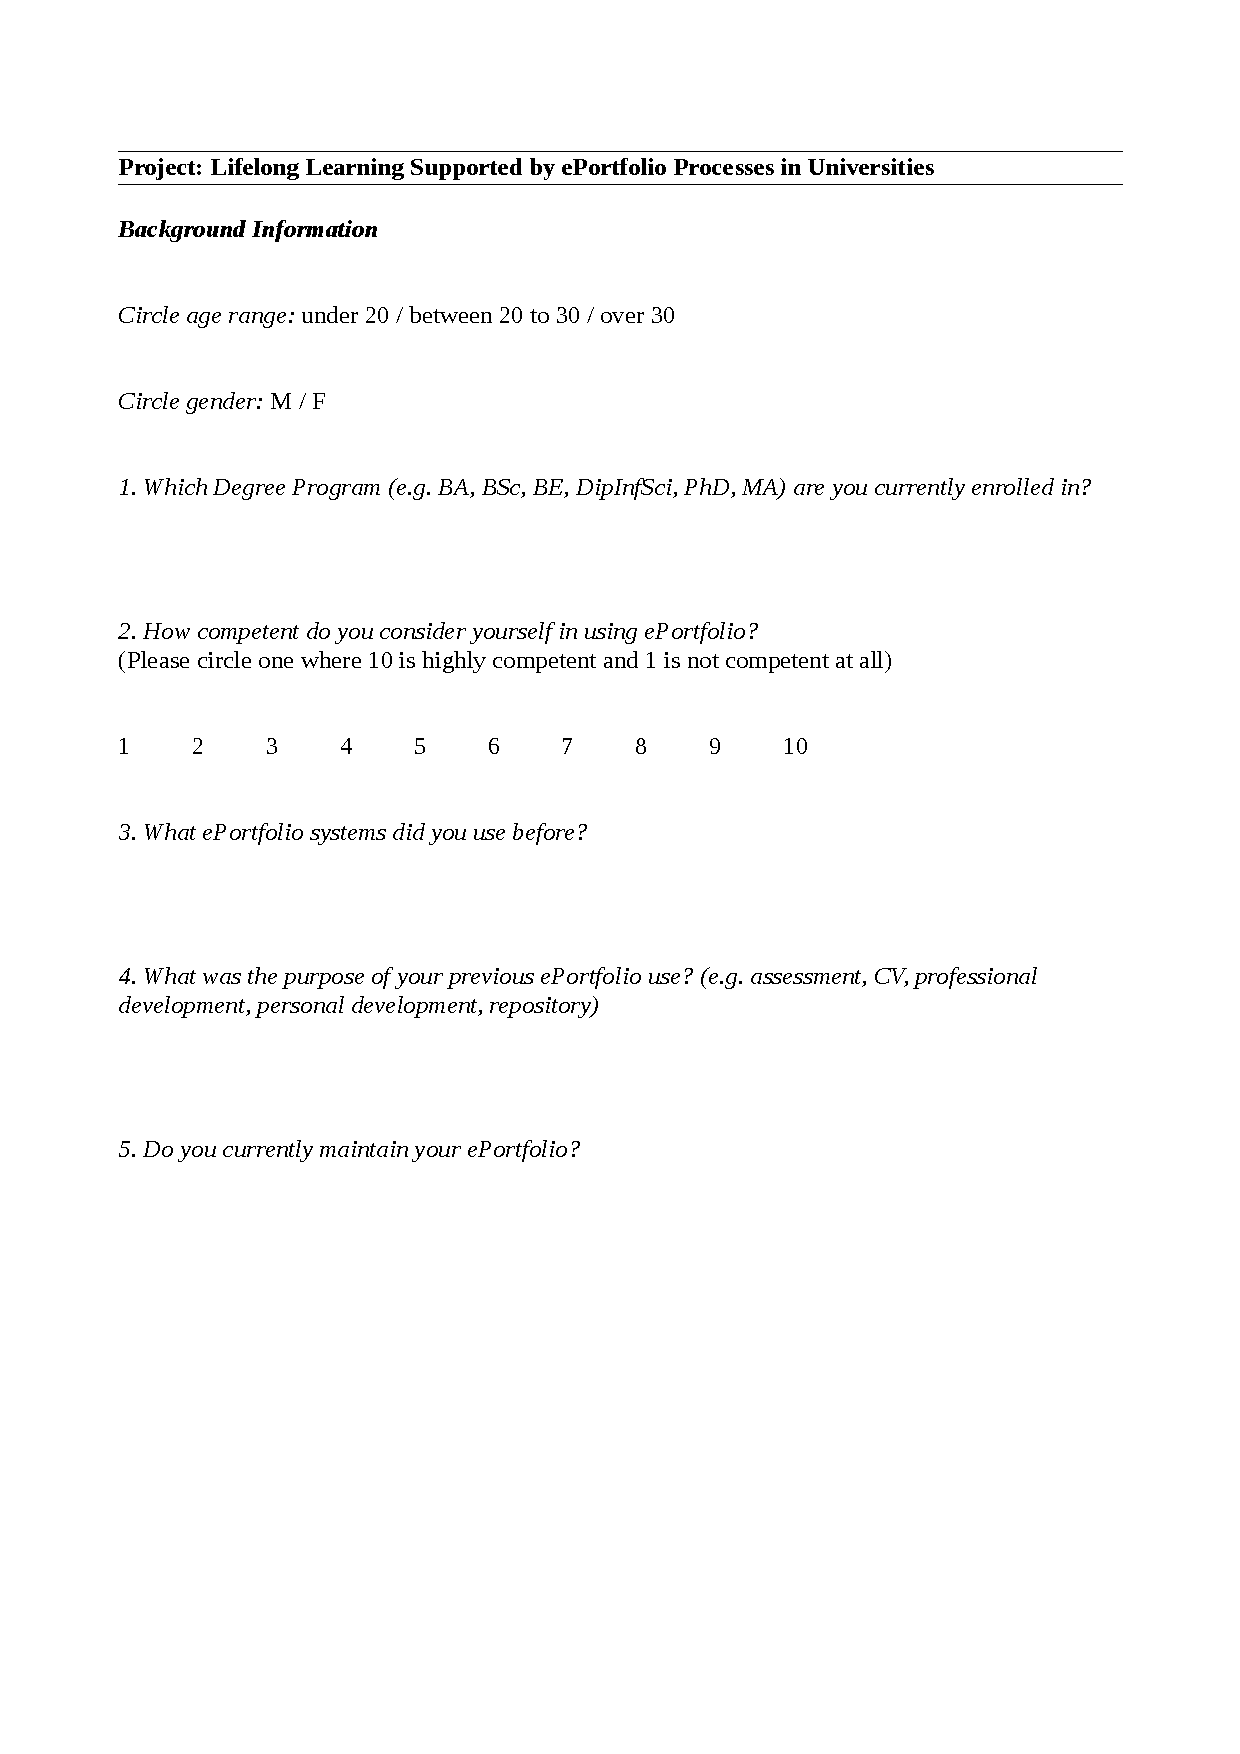
\includepdf[scale=0.7,pages=1,pagecommand=\section{Background
Questionnaire},frame]{appendix/Background-2011.pdf}